\begin{frame}{Ironhide: chains endpoints}

  Ironhide is the component that manages traffic that \textbf{enter and exit}
  from the chain

  \vfill{}

  It classify entering packets choosing the most suitable chain
  \begin{itemize}
    \item Classification based on \textbf{transport layer protocol} used
    \item Performed only at the edges of the chain, not during the traversal
  \end{itemize}

  \vfill{}

  \textbf{Encapsulate/decapsulate} packets to traverse the chain

  \begin{textblock*}{1cm}(11cm, 6cm)
    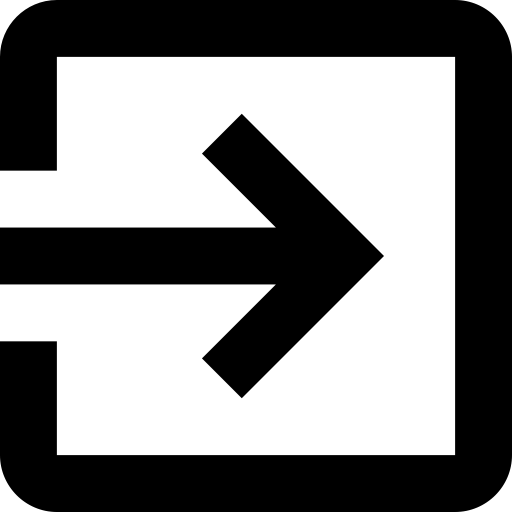
\includegraphics[scale=0.08]{enterexit}
  \end{textblock*}

  \vfill{}

  Keep the connection with the sender/receiver of packets

\end{frame}